%
%	Begrifflichkeiten
%

\pagebreak
\section{NIS2}

\onehalfspacing

\subsection{The Network and Information Security Directive}

The European Commission and the High Representative of the Union for Foreign Affairs and Security Policy presented a new EU Cybersecurity Strategy at the end of 2020.\footnote{See \textit{EU (2023)}: Cybersecurity Policies. \cite{cyberPol}}

\subsubsection{Cybersecurity Across the Union}

\subsubsection{The EU Cybersecurity Agency ENISA}

\subsubsection{Cyber Resilience Act}

\subsubsection{Cybersecurity Act}

\subsubsection{Cyber Solidarity Act}

\subsubsection{Certification}

\subsection{Center for Internet Security}

CISecurity is an acronym for the Center for Internet Security. It's a non-profit organization that helps individuals, businesses, and governments protect themselves from cyber threats. Their key offerings are CIS Controls and CIS Benchmarks.

The Center for Internet Security was founded 20 years ago in Washington, D.C., in response to increased cyber-attacks. It has established itself as the go-to resource for computer security.

Its funding comes from various government and non-profit grant programs designed to improve the overall cybersecurity posture of the U.S. and through the sale of various cybersecurity best practices tools and resources, such as CIS SecureSuite Membership and CIS Hardened Images, and cybersecurity services like CIS Endpoint Security Services.

\subsubsection{CIS Controls}

CIS Controls are actionable and prioritized recommendations that provide organizations with a cybersecurity defense strategy and improve their cybersecurity posture.\footnote{See \textit{CIS (2024)}: Critical Security Controls. \cite{cisControls}}

CIS Controls are organized into Implementation Groups:

\begin{itemize}
    \item IG1 is a minimum standard of information security aimed at all enterprises.
    \item IG2 focuses on enterprises dealing with sensitive client or company information.
    \item IG3 focuses on the impact of zero-day attacks and targeted attacks from sophisticated adversaries and might not be suitable for all enterprises.
\end{itemize}

Implementation groups are cumulative; i.e., to implement IG2, you would also need to implement IG1.

The CIS Controls are a standalone toolset. There are mappings available for other security and compliance requirements, such as ISO 27001, NIST CSF, or NIST SP 800-53.\footnote{See \textit{CIS (2024)}: Critical Controls Mappings. \cite{cisMappings}}

\subsubsection{CIS Benchmarks}

CIS Benchmarks are detailed configuration guidelines for operating systems, hardware, and software. These can be validated and monitored automatically using specialized tools.

The Benchmark itself addresses the CIS Controls safeguards of Secure
Configurations and maintaining a Secure Configuration Process without individual mappings to these safeguards.\footnote{See \textit{CIS (2024)}: Benchmark List. \cite{cisBenchmarks}}

In CIS Controls v8, this would be Control 4.1, "Establish and Maintain a Secure Configuration Process"; in CIS Controls v7, it was Control 5.1, "Establish Secure Configurations." Both Controls are part of the Implementation Group IG1 in their respective version.

No other controls are addressed in the CIS Benchmarks.

\subsection{Rancher}

To easily manage the security of a set of Kubernetes clusters, we can turn to Rancher.

What is Rancher? The Rancher Labs website states it is "[...] a complete software stack for teams adopting containers. It addresses the operational and security challenges of managing multiple Kubernetes clusters while providing DevOps teams with integrated tools for running containerized workloads."\footnote{\textit{Rancher Labs (2019)}: Run Kubernetes Everywhere. \cite{rancher}}

Using a user-friendly GUI, Rancher provides a management platform to manage multiple Kubernetes clusters in Enterprise IT centrally. It also offers application development integration tools and robust enterprise-grade security and governance features. For operations, Rancher provides integrated solutions for logging, monitoring, and auditing, together with many other features, such as CIS scans or a built-in service mesh.

The classic Rancher GUI looks like this:

\begin{figure}[H]
\centering
\caption {Rancher Dashboard}
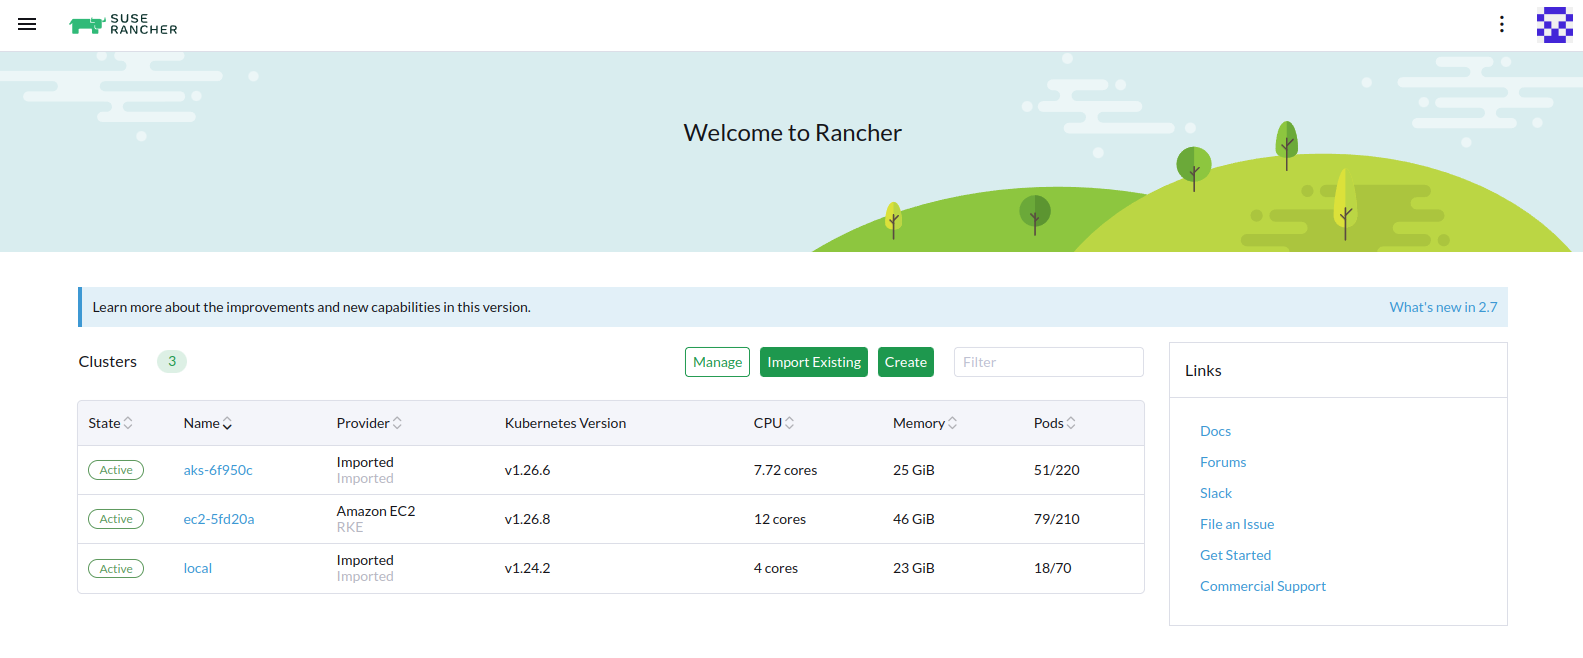
\includegraphics[width=\linewidth]{images/rancher-dashboard.png}
\label{fig:rancherDashboard}
\end{figure}

We will use Rancher's integrated CIS Benchmarks for our further analysis.

\subsubsection{CIS Benchmarks}

\subsubsection{CIS Benchmarks Installation}

\begin{lstlisting}[caption=Installing CIS Benchmarks, frame=single, basicstyle=\ttfamily]
# CIS Benchmarks
resource "rancher2_app_v2" "cisbench_fom" {
  lifecycle {
    ignore_changes = all
  }
  cluster_id = rancher2_cluster.cluster_fom.id
  name = "rancher-cis-benchmark"
  namespace = "cis-operator-system"
  project_id = data.rancher2_project.system.id
  repo_name = "rancher-charts"
  chart_name = "rancher-cis-benchmark"
  chart_version = var.cischart
}
\end{lstlisting}

\subsubsection{CIS Benchmark Reports}

\begin{itemize}
 \item AKS 1.0
 \item Kubernetes 1.6
\end{itemize}
